\documentclass[10pt,landscape]{article}
\usepackage{multicol}
\usepackage{calc}
\usepackage{ifthen}
\usepackage[landscape]{geometry}
\usepackage{amsmath,amsthm,amsfonts,amssymb}
\usepackage{color,graphicx,overpic}
\usepackage{hyperref}


\pdfinfo{
  /Title (example.pdf)
  /Creator (TeX)
  /Producer (pdfTeX 1.40.0)
  /Author (Seamus)
  /Subject (Example)
  /Keywords (pdflatex, latex,pdftex,tex)}

% This sets page margins to .5 inch if using letter paper, and to 1cm
% if using A4 paper. (This probably isn't strictly necessary.)
% If using another size paper, use default 1cm margins.
\ifthenelse{\lengthtest { \paperwidth = 11in}}
    { \geometry{top=.5in,left=.5in,right=.5in,bottom=.5in} }
    {\ifthenelse{ \lengthtest{ \paperwidth = 297mm}}
        {\geometry{top=1cm,left=1cm,right=1cm,bottom=1cm} }
        {\geometry{top=1cm,left=1cm,right=1cm,bottom=1cm} }
    }

% Turn off header and footer
\pagestyle{empty}

% Redefine section commands to use less space
\makeatletter
\renewcommand{\section}{\@startsection{section}{1}{0mm}%
                                {-1ex plus -.5ex minus -.2ex}%
                                {0.5ex plus .2ex}%x
                                {\normalfont\large\bfseries}}
\renewcommand{\subsection}{\@startsection{subsection}{2}{0mm}%
                                {-1explus -.5ex minus -.2ex}%
                                {0.5ex plus .2ex}%
                                {\normalfont\normalsize\bfseries}}
\renewcommand{\subsubsection}{\@startsection{subsubsection}{3}{0mm}%
                                {-1ex plus -.5ex minus -.2ex}%
                                {1ex plus .2ex}%
                                {\normalfont\small\bfseries}}
\makeatother

% Define BibTeX command
\def\BibTeX{{\rm B\kern-.05em{\sc i\kern-.025em b}\kern-.08em
    T\kern-.1667em\lower.7ex\hbox{E}\kern-.125emX}}

% Don't print section numbers
\setcounter{secnumdepth}{0}


\setlength{\parindent}{0pt}
\setlength{\parskip}{0pt plus 0.5ex}

%My Environments
\newtheorem{example}[section]{Example}
% -----------------------------------------------------------------------

\begin{document}
\raggedright
\footnotesize
\begin{multicols}{3}


% multicol parameters
% These lengths are set only within the two main columns
%\setlength{\columnseprule}{0.25pt}
\setlength{\premulticols}{1pt}
\setlength{\postmulticols}{1pt}
\setlength{\multicolsep}{1pt}
\setlength{\columnsep}{2pt}

\begin{center}
     \Large{\underline{Software Modelling and Design}} \\
\end{center}

\section{W1: Use Case Diagrams}
\textbf{Actors:} A person or a system that interacts with the system.\\
\begin{itemize}
    \item \textbf{Primary actor:} initiates the use case. Has goals that influences the purpose of the system under discussion (SuD).
    \item \textbf{Supporting actor:} provides a service to the SuD, like a dependency.
    \item \textbf{Offstage actor:} interacts with the SuD, but is not part of the SuD. Almost like a spectator.
\end{itemize}
\textbf{Use case:} a sequence of actions that provide a measurable value to an actor.\\
\textbf{Use case diagram:} a diagram that shows the actors and use cases of a system.\\
\textbf{How to find useful use cases?}
\begin{itemize}
    \item \textbf{Boss test:} if I told my boss about this use case, would he/she care?
    \item \textbf{Elementary business process (EBP):} a task that is performed by one person, in one place, in response to a business event, and adds measurable business value.
    \item \textbf{Size test:} is a task very seldom a single action/step?
\end{itemize}
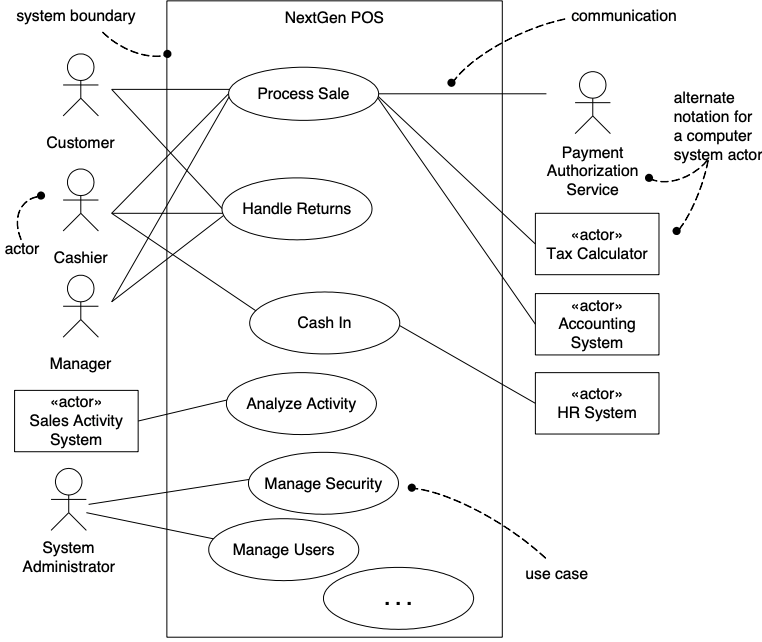
\includegraphics[width=\linewidth]{figs/uml-use-case-diagram.png}
\section{W2: Domain models, SSDs}

\section{W3: Design models, RDDs}

\section{W4-5: GRASP}
\begin{itemize}
    \item \textbf{Creator:} Who should be responsible for creating a new instance of a class?\\
    \textit{Answer} Assign class B responsibility to create instance of class A if one of these is true:
    \begin{itemize}
        \item B contains or compositely aggregates A
        \item B records A
        \item B closely uses A
        \item B has the initialising data that A needs
    \end{itemize}
    \textit{Contraindications} If creation of objects has significant complexity, e.g., using recycled instances for performance, or conditionally creating an instance from one of a family of similar classes based upon some external property value or other context information, then use a Factory pattern instead.
    \item \textbf{Information expert:} Who has the information necessary to fulfil responsibilities?\\
    \textit{Answer} Assign a responsibility to the class that has the information needed to fulfil it.\\
    \textit{Contraindications} In some situations, a solution suggested by Expert is undesirable because of problems with the resulting dependencies.
    \item \textbf{Low coupling:} How can the coupling between two classes be minimised?\\
    \item \textbf{High cohesion:} How can the responsibilities of a class be appropriately assigned to ensure that the class has high cohesion?\\
    \item \textbf{Controller:} What first object beyond the UI layer receives and coordinates (or controls) a system operation?\\
    \textit{Answer} Use a Controller object to deal with major system events.\\
    \textit{Contraindications} If the system operation is simple, and the system has only one or two layers, then the Controller may be unnecessary.
    \item \textbf{Indirection:} How can indirection be used to increase flexibility and reusability?\\
    \textit{Answer} Assign responsibility to an intermediate object to mediate between other components or services to reduce the coupling between them.\\
    \textit{Contraindications} If the indirection adds complexity with little benefit, then it should be avoided.
    \item \textbf{Pure fabrication:} Where can an additional class be inserted that does not represent a problem domain concept, and that has no superclass?\\
    \textit{Answer} Assign a highly cohesive set of responsibilities to an artificial or convenience class that does not represent a problem domain concept.\\
    \textit{Contraindications} If the class is not cohesive, then it should be avoided.
    \item \textbf{Polymorphism:} How can polymorphism be used to simplify client use of entities and reduce coupling? How can we produce reusable code?\\
    \textit{Answer} When there are related behaviour but only differ by the type, assign responsibility for the behaviour using polymorphic operations. Polymorphism can be achieved by using inheritance or interfaces.\\
    \textit{Contraindications} If the use of polymorphism adds complexity with little benefit, then it should be avoided.
    \item \textbf{Protected variations:} How can we design objects, subsystems, and systems so that the variations in those elements that are likely to change are encapsulated in well-defined, stable areas?\\
    \textit{Answer} Identify points of predicted variation and encapsulate them.\\
    \textit{Contraindications} If the use of protected variations adds complexity with little benefit, then it should be avoided.
\end{itemize}

\section{W6: State machines}
State machine is a behaviour model that captures the dynamic behaviour of an object in terms of states, events and state transitions.
\textbf{State:} is the condition of an object at a moment in time.
\textbf{Event:} is a significant or noteworthy occurrence that affects the object to change state.
\textbf{Transition:} is a directed relationship between two states such that an event can cause the object to change from the prior state to the subsequent state.
\textbf{Guard condition:} is a boolean expression that must be true for the transition to occur.
\textbf{Action:} is an operation that is performed when a transition occurs.
\textbf{State-dependent object:} reacts differently to events depending on the object's state.
\textbf{State-independent object:} for all events of interest, an object always reacts to the event the same way.
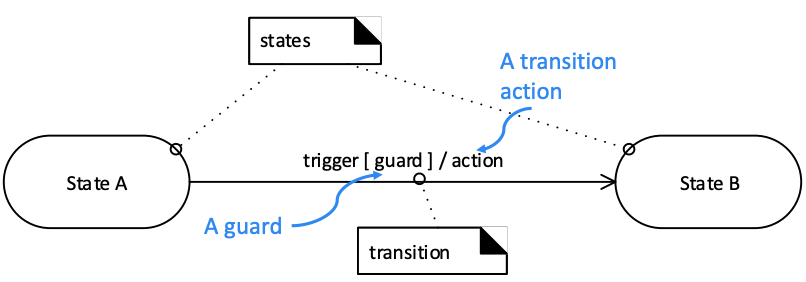
\includegraphics[width=\linewidth]{figs/state-machine.png}
\textbf{Nested state machine:} a state machine that is nested inside another state machine. These are called superstates and substates.
\textbf{Choice pseudostate:} a pseudostate that chooses between two or more transitions.
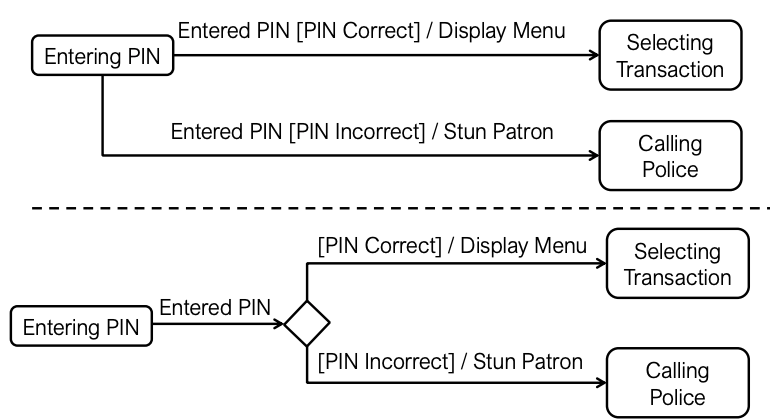
\includegraphics[width=\linewidth]{figs/choice-pseudostate.png}

\section{W7-9: Gang of Four}

\section{W10: Architecture}

\section{W11: Software process}
\textbf{Functional requirements:} describe the functionality or system services that the system must provide.
\textbf{Non-functional requirements:} are constraints on the services or functions offered by the system such as timing constraints, constraints on the development process, standards, etc.
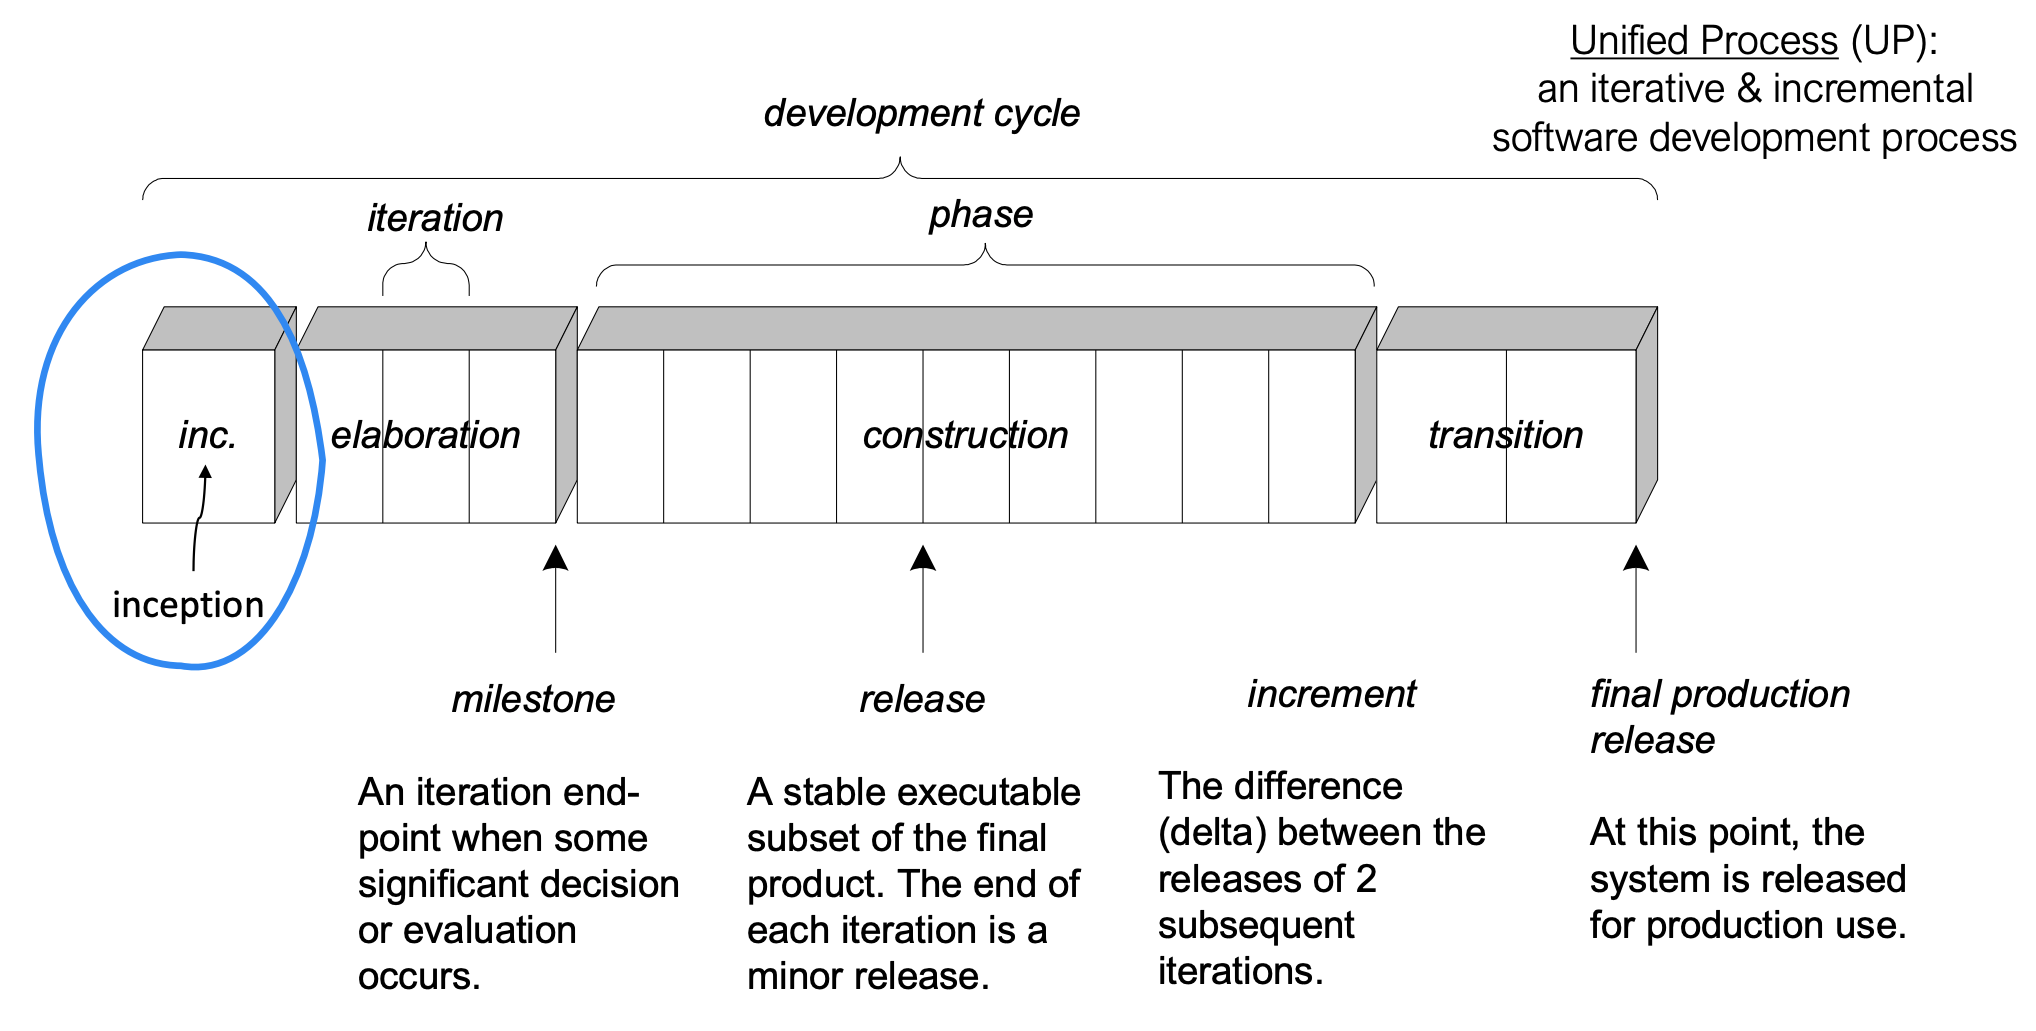
\includegraphics[width=\linewidth]{figs/unified-process.png}
\begin{enumerate}
    \item \textbf{Inception:} establish the business case for the system.
    \item \textbf{Elaboration:} develop an understanding of the problem domain and the system architecture.
    \item \textbf{Construction:} develop the system.
    \item \textbf{Transition:} deploy the system into its operating environment.
\end{enumerate}


% % You can even have references
% \rule{0.3\linewidth}{0.25pt}
% \scriptsize
% \bibliographystyle{abstract}
% \bibliography{refFile}
\end{multicols}
\end{document}